\chapter{Drawing} \label{cap:disegnare}

\section{Moving thje Turtle around – Drawing - Using variables}

\subsection{Basic commands} \label{sec:comandi-fondamentali}

The program allows to create graphics through the movements of a “turtle” who obeys specific commands. Let's just see an example.
Open a new text document and write this command:
\vskip 1cm

\begin{scriptsize}
\begin{minipage}{01.0\textwidth}
\begin{itemize}[itemsep=-3pt,parsep=2pt]
\item[] \hspace{0.5cm} \textbf{HOME} 
\end{itemize}
\end{minipage}
\end{scriptsize}

\vskip 1cm

You'll see that the turtle just appeared in the middle of the screen with its head up:

\begin{figure}[H]
   \centering
   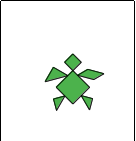
\includegraphics[width=3.0cm,trim=4 4 8 4,clip]{./images/disegnare/disegnare-1.png}
   \label{dis-1}
\end{figure}

Now, add another command (from now on I'll write in bold just the new commands that are being introduced):

\begin{scriptsize}
\begin{minipage}{0.45\textwidth}
\begin{itemize}[itemsep=-3pt,parsep=2pt]
\item[] \hspace{0.5cm} HOME 
\item[] \hspace{0.5cm} \textbf{FORWARD 100}
\end{itemize}
\end{minipage}
\end{scriptsize}
\begin{minipage}{0.5\textwidth}
\begin{figure}[H]
   
\includegraphics[width=3.0cm,trim=4 4 8 4,clip]{./images/disegnare/disegnare-2.png}
   \label{dis-2}
\end{figure}
\end{minipage} \hfill

\vskip 1cm

The turtle has moved, drawing a line; this is the way you can draw by giving commands to the turtle.
Let's now write the following instructions:

\vskip 1cm

\begin{scriptsize}
\begin{minipage}{0.45\textwidth}
\begin{itemize}[itemsep=-3pt,parsep=2pt]
\item[] \hspace{0.5cm} HOME 
\item[] \hspace{0.5cm} FORWARD 100
\item[] \hspace{0.5cm} \textbf{RIGHT 90}
\item[] \hspace{0.5cm} FORWARD 50
\item[] \hspace{0.5cm} \textbf{RIGHT 90}
\item[] \hspace{0.5cm} FORWARD 50
\item[] \hspace{0.5cm} \textbf{RIGHT 90}
\item[] \hspace{0.5cm} FORWARD 50
\item[] \hspace{0.5cm} RIGHT \textbf{90} 
\item[] \hspace{0.5cm} 
\end{itemize}
\end{minipage}
\end{scriptsize}
\begin{minipage}{0.5\textwidth}
\begin{figure}[H]
   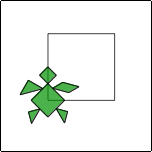
\includegraphics[width=3.0cm,trim=4 4 8 4,clip]{./images/disegnare/disegnare-3.png}
   \label{dis-3}
\end{figure}
\end{minipage} \hfill

\vskip 1cm

We have drawn four sides, and at the end of each side we turned right by 90\degree, thus obtaining a square.
Just two words about the peculiarity of LibreLogo. The sequence of instructions we wrote is a bit of code, it’s a software. We wrote it in a particular kind of language, which is Logo's, and is it also very simple, but it's a software just like any other.
Usually the software is written in special documents using simple text editing and context editing and it’s saved that way.
Then, the computer executes them.
The ways these operations are being executed vary a lot, depending on the kind of languages and the context.
Nowadays there are hundreds of different languages that are used for the most different goals.
The peculiarity of LibreLogo is that the software is written in a document and the turtle “works” on the same document, leaving its mark in a graphic way.
So, one obtains both the code and its graphic result all together in one document.
The graphics can be selected with the mouse and, eventually, may be transferred to various contexts.
For example, I created the above pictures by playing with the turtle in another document, then I selected the graphics and I brought them here. Another notation: a group of instructions made to operate in sequence is called script, expression that we will use profusely.

The interaction between Logo and LibreOffice goes beyond that. It’s evident that when we write this command

\vskip 1cm

\begin{scriptsize}
\begin{minipage}{1.0\textwidth}
\begin{itemize}[itemsep=-3pt,parsep=2pt]
\item[] \hspace{0.5cm} FORWARD 50  
\end{itemize}
\end{minipage}
\end{scriptsize}

\vskip 1cm

the number 50 expresses the length of the path that the turtle needs to make. You can verify this at once by changing the value and watching what the turtle does instead.

But what does that 50 stand for?
They are typographic points: 50 pt. One point is 0.35 mm\footnote {The correct definition is: 1 pt = 1/72 inches, where 1 inch = 25.4 mm. Therefore 1 pt = 2.54/72 = $.352\overline{7}$ mm}. LibreLogo understands unity measurements, so you can write 50, 50pt, 50mm, 50cm, 50in (inches), 50 " ( " stands for inch). They are all different lengths, of course. Let's use mm, for example:

\vskip 1cm

\begin{scriptsize}
\begin{minipage}{0.45\textwidth}
\begin{itemize}[itemsep=-3pt,parsep=2pt]
\item[] \hspace{0.5cm} \textbf{CLEARSCREEN}
\item[] \hspace{0.5cm} HOME
\item[] \hspace{0.5cm} FORWARD \textbf{50mm}
\item[] \hspace{0.5cm} RIGHT 90
\item[] \hspace{0.5cm} FORWARD \textbf{50mm}
\item[] \hspace{0.5cm} RIGHT 90
\item[] \hspace{0.5cm} FORWARD \textbf{50mm}
\item[] \hspace{0.5cm} RIGHT 90
\item[] \hspace{0.5cm} FORWARD \textbf{50mm} 
\item[] \hspace{0.5cm} RIGHT 90     
\end{itemize}
\end{minipage}
\end{scriptsize}
\begin{minipage}{0.5\textwidth}
\begin{figure}[H]
   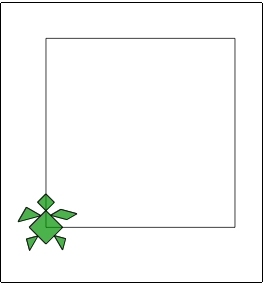
\includegraphics[width=5.0cm,trim=4 4 8 4,clip]{./images/disegnare/disegnare-4.png}
   \label{dis-4}
\end{figure}
\end{minipage} \hfill

\vskip 1cm

The square is obviously bigger because the previous one was 50 pt = 17.6 mm. 
Let's try and make the drawing more complicate, imagining to draw a house. The turtle is located on the bottom left angle, looking upward. 
Firstly, we need to make it go up to the angle on the top left. Let's try, and at the same time, let's take advantage of the fact that the instructions can be conveniently grouped on the same line, if we need it:

\vskip 1cm

\begin{scriptsize}
\begin{minipage}{0.40\textwidth}
\begin{itemize}[itemsep=-3pt,parsep=2pt]
\item[] CLEARSCREEN             
\item[] HOME
\item[] FORWARD 50mm RIGHT 90
\item[] FORWARD 50mm RIGHT 90
\item[] FORWARD 50mm RIGHT 90
\item[] FORWARD 50mm RIGHT 90
\item[] FORWARD 50mm
\end{itemize}
\end{minipage}
\end{scriptsize}
\begin{minipage}{0.4\textwidth}
\begin{figure}[H]
   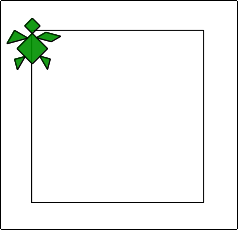
\includegraphics[width=5.0cm,trim=4 4 8 4,clip]{./images/disegnare/disegnare-5.png}
   \label{dis-5}
\end{figure}
\end{minipage} \hfill

\vskip 1cm

There are no strict rules to group instructions on the same line, but it can be useful to read the code easily.
It's vital to get things smooth because, as the code keeps growing, it can rapidly become complicated and all the tricks to make it nice and simple are useful.

\vskip 1cm

\begin{minipage}{0.45\textwidth}

Now we need to build the roof of the house. We can do this by drawing an equilateral triangle over the square, its base coinciding with the upper side of the square. Being equilateral, the other sides of the triangle will have to be 50mm long as well. So, in order to make the left side of the roof, the turtle will need to move 50mm, but before that, it needs to change direction. How much? Since the internal angles of an equilateral triangle are 60\degree each, the turtle needs to detour by 90\degree - 60\degree = 30\degree  on the right. Once it has reached the top, drawing the left side of the roof, it will have to turn right by 120\degree in order to draw the right side. Finally, it will turn by 30\degree  on the right to align itself to the wall of the house.

\end{minipage}
\begin{minipage}{0.5\textwidth}
\begin{figure}[H]
   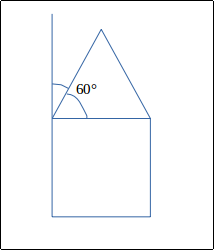
\includegraphics[width=6.5cm,trim=4 4 8 4,clip]{./images/disegnare/disegnare-6.png}
   \label{dis-6}
\end{figure}
\end{minipage} \hfill

\vskip 1cm

\begin{scriptsize}
\begin{minipage}{0.40\textwidth}
\begin{itemize}[itemsep=-3pt,parsep=2pt]
\item[] CLEARSCREEN             
\item[] HOME
\item[] FORWARD 50mm RIGHT 90
\item[] FORWARD 50mm RIGHT 90
\item[] FORWARD 50mm RIGHT 90
\item[] FORWARD 50mm RIGHT 90
\item[] FORWARD 50mm RIGHT 30
\item[] FORWARD 50mm RIGHT 120
\item[] FORWARD 50mm RIGHT 30
\end{itemize}
\end{minipage}
\end{scriptsize}
\begin{minipage}{0.4\textwidth}
\begin{figure}[H]
   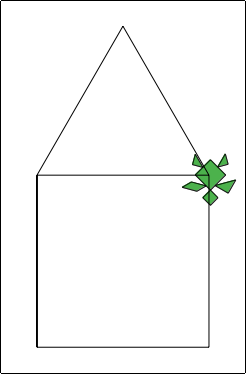
\includegraphics[width=5.0cm,trim=4 4 8 4,clip]{./images/disegnare/disegnare-7.png}
   \label{dis-7}
\end{figure}
\end{minipage} \hfill

\vskip 1cm

Now, let's suppose we want to draw a window in the middle of the wall. To do that it's necessary to introduce two new commands - PENUP and PENDOWN - that allow to move the turtle without drawing.


\vskip 1cm

\begin{scriptsize}
\begin{minipage}{0.40\textwidth}
\begin{itemize}[itemsep=-3pt,parsep=2pt]
\item[] CLEARSCREEN             
\item[] HOME
\item[] FORWARD 50mm RIGHT 90
\item[] FORWARD 50mm RIGHT 90
\item[] FORWARD 50mm RIGHT 90
\item[] FORWARD 50mm RIGHT 90
\item[] FORWARD 50mm RIGHT 30
\item[] FORWARD 50mm RIGHT 120
\item[] FORWARD 50mm RIGHT 120
\item[] \textbf{PENUP}
\item[] FORWARD 50mm/3 LEFT 90
\item[] FORWARD 50mm/3

we underlined red the path that was made without leaving a mark. 

\end{itemize}
\end{minipage}
\end{scriptsize}
\begin{minipage}{0.4\textwidth}
\begin{figure}[H]
   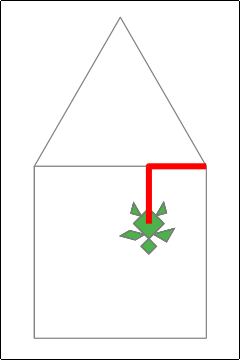
\includegraphics[width=5.0cm,trim=4 4 8 4,clip]{./images/disegnare/disegnare-8.png}
   \label{dis-8}
\end{figure}
\end{minipage} \hfill

\vskip 1cm

\begin{scriptsize}
\begin{minipage}{0.40\textwidth}
\begin{itemize}[itemsep=-3pt,parsep=2pt]
\item[] CLEARSCREEN             
\item[] HOME
\item[] FORWARD 50mm RIGHT 90
\item[] FORWARD 50mm RIGHT 90
\item[] FORWARD 50mm RIGHT 90
\item[] FORWARD 50mm RIGHT 90
\item[] FORWARD 50mm RIGHT 30
\item[] FORWARD 50mm RIGHT 120
\item[] FORWARD 50mm RIGHT 120
\item[] \textbf{PENUP}
\item[] FORWARD 50mm/3 LEFT 90
\item[] FORWARD 50mm/3
\item[] \textbf{PENDOWN}
\item[] FORWARD 50mm/3 RIGHT 90
\item[] FORWARD 50mm/3 RIGHT 90
\item[] FORWARD 50mm/3 RIGHT 90
\item[] FORWARD 50mm/3 RIGHT 90
\end{itemize}
\end{minipage}
\end{scriptsize}
\begin{minipage}{0.4\textwidth}
\begin{figure}[H]
   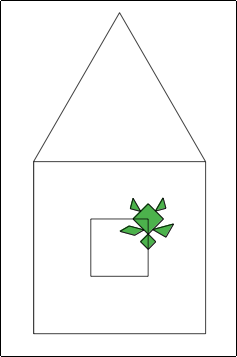
\includegraphics[width=5.0cm,trim=4 4 8 4,clip]{./images/disegnare/disegnare-9.png}
   \label{dis-9}
\end{figure}
\end{minipage} \hfill

\vskip 1cm

Let's try and enrich the drawing further, i.e. using colours.
  

\vskip 1cm

\begin{scriptsize}
\begin{minipage}{0.40\textwidth}
\begin{itemize}[itemsep=-3pt,parsep=2pt]
\item[] CLEARSCREEN             
\item[] HOME
\item[] \textbf{PENCOLOR  "green "}
\item[] FORWARD 50mm RIGHT 90
\item[] FORWARD 50mm RIGHT 90
\item[] FORWARD 50mm RIGHT 90
\item[] FORWARD 50mm RIGHT 90
\item[] FORWARD 50mm RIGHT 30
\item[] \textbf{PENCOLOR  "red "}
\item[] FORWARD 50mm RIGHT 120
\item[] FORWARD 50mm RIGHT 120
\item[] PENUP
\item[] FORWARD 50mm/3
\item[] LEFT 90
\item[] FORWARD 50mm/3
\item[] PENDOWN
\item[] \textbf{PENCOLOR  "blue "}
\item[] FORWARD 50mm/3 RIGHT 90
\item[] FORWARD 50mm/3 RIGHT 90
\item[] FORWARD 50mm/3 RIGHT 90
\item[] FORWARD 50mm/3 RIGHT 90
\item[] \textbf{PENCOLOR  "gray "}
\end{itemize}
\end{minipage}
\end{scriptsize}
\begin{minipage}{0.4\textwidth}
\begin{figure}[H]
   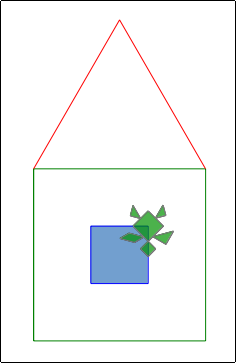
\includegraphics[width=5.0cm,trim=4 4 8 4,clip]{./images/disegnare/disegnare-10.png}
   \label{dis-10}
\end{figure}
\end{minipage} \hfill

\vskip 1cm

And why not colour the inside as well?


\vskip 1cm

\begin{scriptsize}
\begin{minipage}{0.40\textwidth}
\begin{itemize}[itemsep=-3pt,parsep=2pt]
\item[] CLEARSCREEN            
\item[] HOME
\item[] FORWARD 50mm RIGHT 90
\item[] FORWARD 50mm RIGHT 90
\item[] FORWARD 50mm RIGHT 90
\item[] FORWARD 50mm RIGHT 90
\item[] FORWARD 50mm RIGHT 30
\item[] \textbf{FILLCOLOR  "yellow " FILL}
\item[] FORWARD 50mm RIGHT 120
\item[] FORWARD 50mm RIGHT 120
\item[] PENUP
\item[] FORWARD 50mm/3
\item[] LEFT 90
\item[] FORWARD 50mm/3
\item[] PENDOWN
\item[] \textbf{FILLCOLOR  "red " FILL}
\item[] FORWARD 50mm/3 RIGHT 90
\item[] FORWARD 50mm/3 RIGHT 90
\item[] FORWARD 50mm/3 RIGHT 90
\item[] FORWARD 50mm/3 RIGHT 90
\item[] \textbf{FILLCOLOR  "green " FILL}
\end{itemize}
\end{minipage}
\end{scriptsize}
\begin{minipage}{0.4\textwidth}
\begin{figure}[H]
   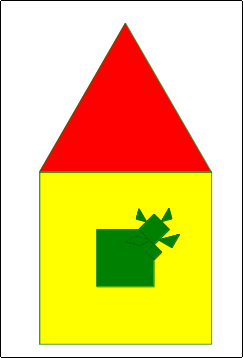
\includegraphics[width=5.0cm,trim=4 4 8 4,clip]{./images/disegnare/disegnare-11.png}
   \label{dis-11}
\end{figure}
\end{minipage} \hfill

\vskip 1cm

In this case as well we used the grouping of instructions:

FILLCOLOR  "green " FILL. With the first one we establish which colour to use
(FILLCOLOR  "green ") and with the second one we proceed to colour the picture - it comes natural to gather them together in one instruction.

The instruction FILL does two things, actually: it closes one picture and it fills it with a colour. 
Let's try:


\vskip 1cm

\begin{scriptsize}
\begin{minipage}{0.40\textwidth}
\begin{itemize}[itemsep=-3pt,parsep=2pt]
\item[] FORWARD 30mm RIGHT 90
\item[] FORWARD 30mm RIGHT 90
\end{itemize}
\end{minipage}
\end{scriptsize}
\begin{minipage}{0.4\textwidth}
\begin{figure}[H]
   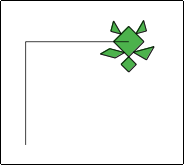
\includegraphics[width=5.0cm,trim=4 4 8 4,clip]{./images/disegnare/disegnare-12.png}
   \label{dis-12}
\end{figure}
\end{minipage} \hfill

\vskip 1cm

This way we have drawn an open picture. If we want to make a triangle, we may let the turtle draw the third side. Alternatively, we may close the picture with FILL, as seen before:

\vskip 1cm

\begin{scriptsize}
\begin{minipage}{0.40\textwidth}
\begin{itemize}[itemsep=-3pt,parsep=2pt]
\item[] FORWARD 30mm RIGHT 90
\item[] FORWARD 30mm RIGHT 90
\item[] FILL                  
\end{itemize}
\end{minipage}
\end{scriptsize}
\begin{minipage}{0.4\textwidth}
\begin{figure}[H]
   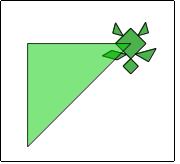
\includegraphics[width=5.0cm,trim=4 4 8 4,clip]{./images/disegnare/disegnare-13.png}
   \label{dis-13}
\end{figure}
\end{minipage} \hfill

\vskip 1cm

This way, the picture has been closed and coloured. We may even close it without colouring it, using the instruction 
 \textbf{CLOSE}:

\vskip 1cm

\begin{scriptsize}
\begin{minipage}{0.40\textwidth}
\begin{itemize}[itemsep=-3pt,parsep=2pt]
\item[] FORWARD 30mm RIGHT 90
\item[] FORWARD 30mm RIGHT 90
\item[] CLOSE                  
\end{itemize}
\end{minipage}
\end{scriptsize}
\begin{minipage}{0.4\textwidth}
\begin{figure}[H]
   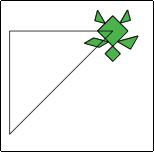
\includegraphics[width=5.0cm,trim=4 4 8 4,clip]{./images/disegnare/disegnare-14.png}
   \label{dis-14}
\end{figure}
\end{minipage} \hfill

\vskip 1cm

It's interesting to notice that, both with FILL and CLOSE, the picture is closed without moving the turtle. So, if we keep adding further moves, they will take place from the turtle's position, that in the previous examples has remains with its head pointing downward.
Let's try and set the two previous code blocks one after the other:

\vskip 1cm

\begin{scriptsize}
\begin{minipage}{0.40\textwidth}
\begin{itemize}[itemsep=-3pt,parsep=2pt]
\item[] FORWARD 30mm RIGHT 90
\item[] FORWARD 30mm RIGHT 90
\item[] FILL                  
\item[] FORWARD 30mm RIGHT 90
\item[] FORWARD 30mm RIGHT 90
\item[] CLOSE                  
\end{itemize}
\end{minipage}
\end{scriptsize}
\begin{minipage}{0.4\textwidth}
\begin{figure}[H]
   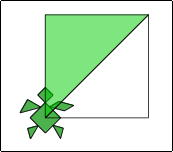
\includegraphics[width=5.0cm,trim=4 4 8 4,clip]{./images/disegnare/disegnare-15.png}
   \label{dis-15}
\end{figure}
\end{minipage} \hfill

\vskip 1cm

After closing and colouring green the upper triangle, the turtle, with the following FORWARD instructions, proceedes to draw two sides of the lower triangle. The instruction CLOSE makes close this second triangle without colouring it.
What if one would want to remove the turtle once the picture is finished? Easy: just add at the end the instruction
 \textbf{HIDETURTLE}. Try! 

\subsection{RGB codes for making colors}

In the previous examples we used codes to express colours, for instance "red". It's possible to name 24 colours:

\vskip 1cm

\begin{figure}[H]
   \centering
   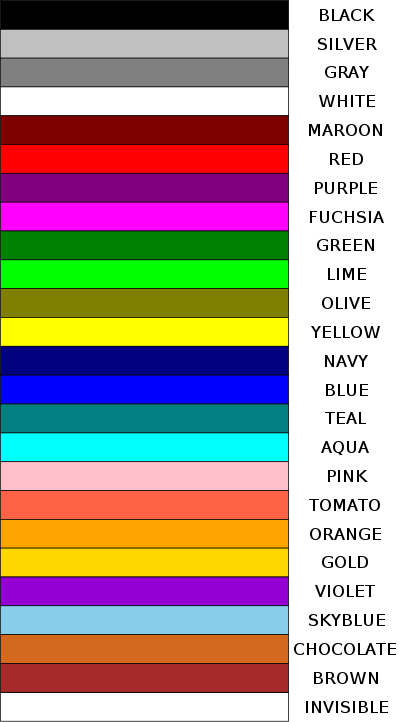
\includegraphics[width=8.0cm,trim=4 4 8 4,clip]{./images/disegnare/disegnare-16.png}
   \label{dis-16-a}
\end{figure}

Actually the available colours are many more. They can be expressed through the so called RGB code, that stands for Red, Green, Blue.
In computer graphics colours can be expressed as a combination of three main colours, which are precisely red, green and blue.
All the others may be expressed by mixing and dosing properly these three basic colours. In order to do that, the intensity of every colour is expressed with a number that goes from 0 to 255 and they are mixed by writing for instance [255,0,0] for red, [0,255,0] for green or [0,0,255] for blue. All the other colours are obtained by varying the parameters inside the square brackets. With [0, 0, 0]  one obtains black and with [255, 255, 255] white. This code is used in any of the commands that allow to specify the colour. For example

PENCOLOR [45, 88, 200]
FILLCOLOR [255, 200, 100]

Just play for a while with these numbers and see which colours come out.

The colours wheel shown above has an oddity: there are two elements with different name but the colour seems the same. Found them? They actually differ, but because of a fourth attribute, which is transparency. Let's see while playing along.

To make things easier, we'll anticipate a new command. In the previous examples we already drew a square, using the instructions FORWARD and RIGHT, conveniently combined. In reality, in order to draw the main geometric shapes, in Logo there are pre-established instructions, that help us write the code synthetically. The square is one of these. In order to make a 50mm side square you write:


\vskip 1cm

\begin{scriptsize}
\begin{minipage}{0.40\textwidth}
\begin{itemize}[itemsep=-3pt,parsep=2pt]
\item[] CLEARSCREEN
\item[] HOME
\item[] \textbf{SQUARE(30mm)}                            
\end{itemize}
\end{minipage}
\end{scriptsize}
\begin{minipage}{0.4\textwidth}
\begin{figure}[H]
   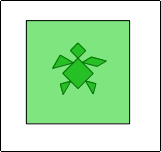
\includegraphics[width=5.0cm,trim=4 4 8 4,clip]{./images/disegnare/disegnare-17.png}
   \label{dis-16-b}
\end{figure}
\end{minipage} \hfill

\vskip 1cm

This way the turtle draws a square, then places itself in the cetre with its head upward (we didn't choose the colour, but it came out "automatically", by default). Let's use this instruction, first to draw a square that we’ll colour red, then we’ll move a bit right down, to draw a second square, making it overlap a little to the previous one, then we’ll colour it white.


\vskip 1cm

\begin{scriptsize}
\begin{minipage}{0.40\textwidth}
\begin{itemize}[itemsep=-3pt,parsep=2pt]
\item[] CLEARSCREEN
\item[] HOME
\item[] FILLCOLOR [255, 0, 0]                                
\item[] SQUARE(50mm)
\item[] FORWARD -25mm
\item[] RIGHT 90                                             
\item[] FORWARD 25mm
\item[] FILLCOLOR [255, 255, 255]
\item[] SQUARE(50mm)                                         
\end{itemize}
\end{minipage}
\end{scriptsize}
\begin{minipage}{0.4\textwidth}
\begin{figure}[H]
   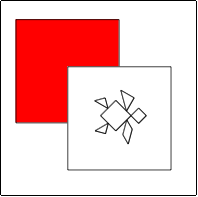
\includegraphics[width=5.0cm,trim=4 4 8 4,clip]{./images/disegnare/disegnare-18.png}
   \label{dis-17}
\end{figure}
\end{minipage} \hfill

\vskip 1cm

Good, now the white square overlapped to the red one. A foreseeable result: the colours overlap because they are opaque. A painter would say that they "cover". Actually, with RGB codes in Logo you can assign a fourth parameter: the "transparency", that you may want to give to a certain colour. With a value 0 you give complete opacity, whilst the value 250 makes it completely transparent. With values between 0 and 250 you can obtain different levels of transparency. So, let's try and make the white square transparent, adding the fourth parameter equal to 255:

\vskip 1cm

\begin{scriptsize}
\begin{minipage}{0.40\textwidth}
\begin{itemize}[itemsep=-3pt,parsep=2pt]
\item[] CLEARSCREEN
\item[] HOME
\item[] FILLCOLOR [255, 0, 0]                                
\item[] SQUARE(50mm)
\item[] FORWARD -25mm
\item[] RIGHT 90                                             
\item[] FORWARD 25mm
\item[] FILLCOLOR [255, 255, 255, 255]
\item[] SQUARE(50mm)                                        
\end{itemize}
\end{minipage}
\end{scriptsize}
\begin{minipage}{0.4\textwidth}
\begin{figure}[H]
   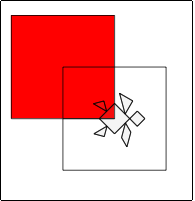
\includegraphics[width=5.0cm,trim=4 4 8 4,clip]{./images/disegnare/disegnare-19.png}
   \label{dis-18}
\end{figure}
\end{minipage} \hfill

\vskip 1cm

The white square has become transparent. If, instead of FILLCOLOR [255, 255, 255, 255] we would have used FILLCOLOR  "invisible ", then we would have obtained the same result. That's the difference between "white" and "invisible", in the colour wheel we saw at the beginning.
One last remark. Looking closely, you can see that in these pictures our turtle have different colours. In fact, the turtle is coloured with the same colour we selected to fill the last picture, maybe with a different transparency. After drawing the square light green, the turtle came out a shade darker. After the white square, it came out light grey and after the invisible colour it came out dark grey. This behaviour does not affect the results we want to obtain because, should we want to use the graphics we are producing in any possible way, in the end we'll just need to add the instruction HIDETURTLE.

\subsection{More commands}

With these basic commands seen so far, it is possible to produce a large amount of graphics. In Logo however there are commands that allow to shorten the picture of some basic forms. We already anticipated the instrution SQUARE that allows to build a square at once. The others are RECTANGLE, CIRCLE and ELLIPSE.
Let's try the following commands:

\vskip 1cm

\begin{scriptsize}
\begin{scriptsize}
\begin{minipage}{0.40\textwidth}
\begin{itemize}[itemsep=-3pt,parsep=2pt]
\item[] CLEARSCREEN
\item[] HOME
\item[] SQUARE 50                               
\item[] CIRCLE 50                                       
\end{itemize}
\end{minipage}
\end{scriptsize}
\end{scriptsize}
\begin{minipage}{0.4\textwidth}
\begin{figure}[H]
   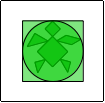
\includegraphics[width=3.0cm,trim=4 4 8 4,clip]{./images/disegnare/disegnare-20.png}
   \label{dis-19}
\end{figure}
\end{minipage} \hfill

\vskip 1cm

You'll see how drawing two pictures in sequence has the effect of overlapping them and making the symmetry centre coincide, and how the turtle always repositions itself on that centre. It’s also evident how the topic\footnote {by "topic" it is intended the value that a command requires to be operated. There can be more than one topic - we'll see some examples} of command SQUARE represents the square's side and the topic of command CIRCLE represents the circle's diameter that we want to build.


\vskip 1cm

\begin{minipage}{0.40\textwidth}

Try and practise with the commands SQUARE and CIRCLE, for instance by building this locomotive. You may practise to respect the given proportions, like those in the example, where the side of the bigger square is two or three times bigger than the smaller squares and the circles' diameter is the same length of the side of the smallest square. You'll find the solution on the next page, but first try to work it out on your own.
 
\end{minipage}
\begin{minipage}{0.4\textwidth}
\begin{figure}[H]
   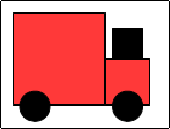
\includegraphics[width=5.0cm,trim=4 4 8 4,clip]{./images/disegnare/disegnare-21.png}
   \label{dis-20}
\end{figure}
\end{minipage} \hfill

\vskip 1cm


One important thing to understand with the code is that the same goal can be achieved in many different ways. There's no absolute criterion to establish the best procedure. Therefore there is no "right answer". One procedure may be better than another on a certain point of view: clarity of the written code, fastness of execution, total memory used from the code, management of possible resources etc. It can happen that a very good code under one of these terms may result a very bad one on another.
 

\newpage

\begin{scriptsize}
\begin{minipage}{0.40\textwidth}
\begin{itemize}[itemsep=-3pt,parsep=2pt]
\item[] COLOR  "red " 
\item[] SQUARE 60 
\item[] PENUP BACK 15 RIGHT 90 FORWARD 45                      
\item[] LEFT 90 PENDOWN 
\item[] SQUARE 30 
\item[] PENUP FORWARD 25 PENDOWN 
\item[] FILLCOLOR  "black "                      
\item[] SQUARE 20 
\item[] PENUP BACK 40 PENDOWN 
\item[] CIRCLE 20                                              
\item[] PENUP LEFT 90 FORWARD 60 PENDOWN 
\item[] CIRCLE 20
\item[] HIDETURTLE                                            
\end{itemize}
\end{minipage}
\end{scriptsize}

\vskip 1cm


The square and the circle need just one parameter to be executed. Instead, the rectangle and ellipse need two parameters. As for the rectangle, the two parameters are the length of the long side and the short side. The instruction to build the rectangle is the following:

\textbf{RECTANGLE [60,40]}

This command produces a rectangle 60 points large and another of 40. In comparison to the square and the circle's cases, this command has another peculiarity: in this case, in order to give the two needed parameters, we recoursed to the writing \textbf{[60,40]}. This is a "list" of values. It's a way of considering a bunch of values as a whole, a list in fact, and the way to obtain this result is to list the values, split them with commas and close them between square brackets. The lists may be useful in various circumstances, not only in this case, but we'll see how later.

\textbf{Esercizio}: try to make a figure like the one below

\vskip 1cm

\begin{figure}[H]
   \centering
   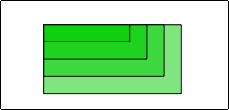
\includegraphics[width=4.0cm,trim=4 4 8 4,clip]{./images/disegnare/disegnare-22.png}
   \label{dis-21}
\end{figure}

\vskip 1cm

In this case as well, try on your own. Then, scroll down the page to see a new way of solving it.

\pagebreak

\vskip 1cm
\begin{scriptsize}
\begin{minipage}{1.0\textwidth}
\begin{itemize}[itemsep=-3pt,parsep=2pt]
\item[] RECTANGLE [40mm, 20mm]
\item[] PENUP FORWARD 2,5mm LEFT 90
\item[] FORWARD 2,5mm RIGHT 90 PENDOWN   
\item[] RECTANGLE [35mm, 15mm]
\item[] PENUP FORWARD 2,5mm LEFT 90
\item[] FORWARD 2,5mm RIGHT 90 PENDOWN
\item[] RECTANGLE [30mm, 10mm]
\item[] PENUP FORWARD 2,5mm LEFT 90      
\item[] FORWARD 2,5mm RIGHT 90 PENDOWN
\item[] RECTANGLE [25mm, 5mm]
\item[] HIDETURTLE                      
\end{itemize}
\end{minipage}
\end{scriptsize}

\vskip 1cm

Another picture that can come in handy is the ellipse. To put it simple, the ellipse is a flattened circle. It's perfectly in the spirit of the Turtle's geometry to get help by using physical activities references: probably the best way of using modern technologies is to keep on using the traditional ones, making the most out of both by integrating them.
Nothing better than to get a little help from Emma Castelnuovo\cite{Castelnuovo}, who writes about the emerging of the ellipse while studying isoperimetrical triangles with same base. Here is the whole writing, in order to respect Emma's valuable didactic intent:

\begin{quote}
Another mathematical subject, as the study of isoperimetrical triangles with the same base, brings us to ponder what we have in front of us.
The material is, even this time, a piece of string. 

In order to build triangles with same base and same perimeter, we'll do it this way: let's fix two nails - A and B - on a table over which has been laid a sheet of paper; AB will be our triangles base. Let's tie both ends of a string to the nails, bearing in mind that the string needs to be wider than the AB side. Let's make sure, with the aid of a pencil, that the string stays stretched and... let the pencil lead us.

This pencil, guided by the string, will draw on the paper an oval shaped curve: it's an ellipse. The points A and B are the focuses of the ellipses. Therefore: the isoperimetrical triangles tops with same base are on an ellipse.
A geometry problem led us to the drawing of the ellipse. With the same string we can make a more or less "flat" ellipse, depending on the distance between the points A and B. We can obtain a circle, if these two points coincide: the circle, actually, is a particular type of ellipse.
  
We find the ellipse again on the street, after dealing with it in geometry problems, when we "step" over it (a street sign's shadow makes an ellipse). In our hectic lives, we rarely pause to notice the shadow that the sun or a lamp cast over an object. Yet now a geometry activity prompts us to look closely and it's indeed the comparison between the shadow cast from the sun or a lamp that arouses our observation skill.

Let's take, for instance, two pencils vertically laid on a table. If they are lit by the sun, their shadow tend to be parallel; on the contrary, if they are lit by a lamp, then their shadows divert.

Hence the mathematical study of affine transformations and projective transformations, to reach perspective, art, the way one looks at a painting, at history.
It's a small geometry problem that challenged to observe and to ... take a look around.


\vskip 1cm

\begin{figure}[H]
   \centering
   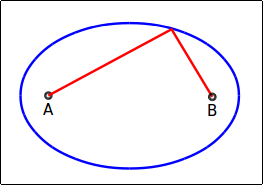
\includegraphics[width=8.0cm,trim=4 4 8 4,clip]{./images/disegnare/disegnare-23.png}
   \label{dis-22}
\end{figure}

\vskip 1cm

\end{quote}

In LibreLogo the ellipse is drawn with the command

\vskip 1cm

\begin{scriptsize}
\begin{minipage}{0.40\textwidth}
\begin{itemize}[itemsep=-3pt,parsep=2pt]
\item[] \textbf{ELLIPSE[40, 20]}
\end{itemize}
\end{minipage}
\end{scriptsize}

\vskip 1cm

Obviously the ellipse does not have a fixed diameter, like the circle. For this reason, to be defined it requires two parameters: the two axis, bigger and smaller. In the example the ellipse has the major axis equal to 60 points and the minor equal to 40 points. It's possible to combine various forms and adjust their parameters to obtain a variety of effects. For instance, a circle inscribed in a square can be obtained also by starting from the instructions to draw rectangles and ellipses:

\vskip 1cm

\begin{scriptsize}
\begin{minipage}{0.40\textwidth}
\begin{itemize}[itemsep=-3pt,parsep=2pt]
\item[] RECTANGLE [60, 60] 
\item[] ELLIPSE [60, 60]   
\end{itemize}
\end{minipage}
\end{scriptsize}

\vskip 1cm

Try to draw a figure like this one:

\vskip 1cm

\begin{figure}[H]
   \centering
   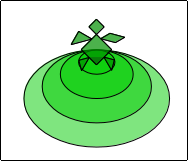
\includegraphics[width=4.0cm,trim=4 4 8 4,clip]{./images/disegnare/disegnare-24.png}
   \label{dis-23}
\end{figure}

\vskip 1cm
\pagebreak

Possibile answer:

\vskip 1cm

\begin{scriptsize}
\begin{minipage}{0.40\textwidth}
\begin{itemize}[itemsep=-3pt,parsep=2pt]
\item[] ELLIPSE [120, 80] 
\item[] PENUP FORWARD 10 PENDOWN
\item[] ELLIPSE [90, 60]         
\item[] PENUP FORWARD 10 PENDOWN
\item[] ELLIPSE [60, 40] 
\item[] PENUP FORWARD 10 PENDOWN
\item[] ELLIPSE [30, 20] 
\item[] PENUP FORWARD 10 PENDOWN 
\end{itemize}
\end{minipage}
\end{scriptsize}

\vskip 1cm

These instructions also allow to use other parameters to obtain rectangular and ellipsis variables. In the case of rectangulars it's possible to adjust a third parameter in order to make the tops rounded:

\vskip 1cm

\begin{scriptsize}
\begin{minipage}{0.40\textwidth}
\begin{itemize}[itemsep=-3pt,parsep=2pt]
\item[] RECTANGLE [60, 50, \textbf{10}]
\end{itemize}
\end{minipage}
\end{scriptsize}
\begin{minipage}{0.4\textwidth}
\begin{figure}[H]
   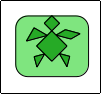
\includegraphics[width=3.0cm,trim=4 4 8 4,clip]{./images/disegnare/disegnare-25.png}
   \label{dis-24}
\end{figure}
\end{minipage} \hfill

\vskip 1cm

Now, let's suppose that a friend just told us about this opportunity, but he can’t remember anything else. Can we control the "roundness" of the tops? Probably with that third parameter our friend told us about, fixing it to 10 value, but how does it work? This is a great example to highlight the crucial tool of software developers: experimentation. So, in this case, we could make some attempts, that we might summarize like this:


\vskip 1cm

\begin{scriptsize}
\begin{minipage}{0.40\textwidth}
\begin{itemize}[itemsep=-3pt,parsep=2pt]
\item[] FILLCOLOR  "invisible " 
\item[] PENCOLOR  "green " 
\item[] RECTANGLE [200, 150, 0] 
\item[] PENCOLOR  "black " 
\item[] RECTANGLE [200, 150, 10] 
\item[] RECTANGLE [200, 150, 20] 
\item[] RECTANGLE [200, 150, 30] 
\item[] RECTANGLE [200, 150, 40] 
\item[] RECTANGLE [200, 150, 50] 
\item[] RECTANGLE [200, 150, 60] 
\item[] RECTANGLE [200, 150, 70] 
\item[] RECTANGLE [200, 150, 80] 
\item[] RECTANGLE [200, 150, 90] 
\item[] RECTANGLE [200, 150, 100] 
\item[] PENCOLOR  "red " 
\item[] ELLIPSE [200,150]          
\end{itemize}
\end{minipage}
\end{scriptsize}
\begin{minipage}{0.4\textwidth}
\begin{figure}[H]
   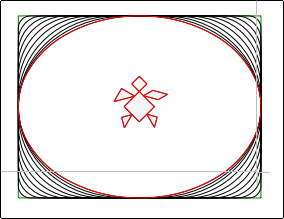
\includegraphics[width=5.0cm,trim=4 4 8 4,clip]{./images/disegnare/disegnare-26.png}
   \label{dis-25}
\end{figure}
\end{minipage} \hfill

\vskip 1cm
 
This way we worked out how to control rounded rectangles. We also realized that, playing with the third parameter, we can wander from the extreme case of a normal rectangle to the real ellipse.
Let's see now the possible variables for the instruction ELLIPSE.

\vskip 1cm

\begin{figure}[H]
   \centering
   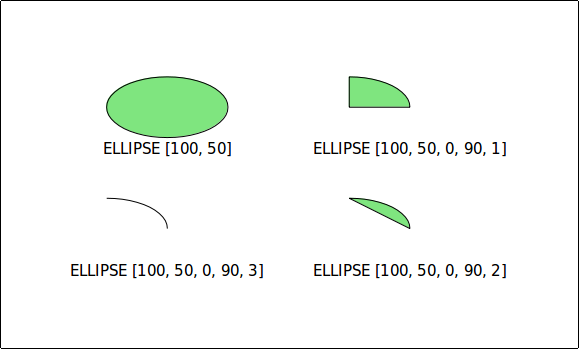
\includegraphics[width=10.0cm,trim=8 8 8 8,clip]{./images/disegnare/disegnare-27.png}
   \label{dis-26}
\end{figure}

\vskip 1cm

In the instruction ELLIPSE we can use 3 additional parameters, that we need to draw just one area of the ellipse. The first two represent the initial and final angle, expressed in degrees, that limit the area. In the above example, having chosen 0 and 90 we established to draw the first quadrant of the ellipse. The fourth parameter establishes if we want to draw one setor of the ellipse (1), one segment of the ellipse (2) or just an arch (3).

\subsection{Variables} \label{sec:variabili}

 
 The instructions we have seen so far allow us to do many things: we learned to move the turtle anywhere around the screen, to make it draw or not, we saw how to control the colour of the line and the filling of figures. We may get the impression that, to make graphics, we won't need more. Instead we just scratched the surface of potentialities of a programming language, even if for educational purposes, as in Logo and its derived.
 We'll introduce the main characteristics as we go. The first of which, that we need at once to get going, is the concept of "variable". So far we used various instructions that require "arguments". the argument is the value that an instruction may require to be executed. For instance the instruction FORWARD wouldn't make any sense without an argument that represents the distance that the turtle needs to cover. The expression FORWARD 50 means that the turtle has to move forward by 50 points; 50 is the value of the argument.
 There are also instructions that require more than an one argument, for example the RECTANGLE and ELLIPSE. 
 Anyway, in all the examples seen before we always used numerical arguments for all the instructions. Actually, all languages allow to make use of an important generalization that's the use of "variables". It’s about symbolic names that can be assigned to convenient numerical values. Let's try and execute the following code:
 

\vskip 1cm

\begin{scriptsize}
\begin{minipage}{0.40\textwidth}
\begin{itemize}[itemsep=-3pt,parsep=2pt]
\item[] CLEARSCREEN
\item[] HOME
\item[] 
\item[] LATO = 100
\item[] ANGOLO = 90
\item[] 
\item[] FORWARD LATO
\item[] LEFT ANGOLO
\item[] FORWARD LATO
\item[] LEFT ANGOLO
\item[] FORWARD LATO
\item[] LEFT ANGOLO
\item[] FORWARD LATO
\item[] HIDETURTLE    
\end{itemize}
\end{minipage}
\end{scriptsize}
\begin{minipage}{0.4\textwidth}
\begin{figure}[H]
   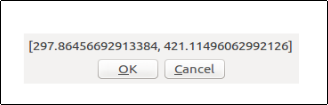
\includegraphics[width=3.0cm,trim=4 4 8 4,clip]{./images/disegnare/disegnare-28.png}
   \label{dis-27}
\end{figure}
\end{minipage} \hfill

\vskip 1cm

We have drawn a square, but instead of using directly the value 100 as an argument of the instructions FORWARD, first we assigned the value 100 to the variable named "SIDE" and then we used this as an argument of all the instructions FORWARD. It's evident which will be the utility of this method: let's suppose I'm not satisfied of this square's dimensions and that I want to try other values of the side. Well, I just need to change the value 100 in the instruction SIDE=100, changing it for example with SIDE=150. Feel free to experiment! You may even want to change the value of ANGLE, trying out different values...
For those who studied algebra basics, they will certainly have recognized the concept of variable, that in that discipline is being used widely to make simple symbolic calculus. They will also remember that the concept of variable is used in various ways, to express quantities that are considered variables - for instance a dependant variable in function of other independent variables - then quantities that we assume constant, finally quantities that assume the meaning of parameters, that are like constant we may be interested to change from time to time.
In any case, all these quantities are being represented in a symbolic way. Actually, those who had time to deepen algebra studies, they will know that the concept of variable is passable of a series of generalizations. No fear, this is not a Maths class in disguise, or maybe it is, in a way: after all Logo represents Seymour Papert's goal to make Maths more accessible.
 
 But what we are doing here does not require special attitudes or skills. We are just introducing one of the possible generalizations, that we are going to need at once. The generalization we are proposing concerns the concept of the turtle's position on the screen.
  The position along aline is determined by a simple number - for instance the position along a road: "Workroads at km...". A different case is that of the position on a surface. In a sat nav, which everybody knows about, you can give the position in geographic terms, but this has to be given through two values: latitude and longitude, denoting the parallel and the meridian. In order to sink a boat at a naval battle board game, you must give two coordinates, for instance b7, where "b represents the column and 7 the line". Likewise you identify cells on a spreadsheet, and so on. Our turtle as well needs two values in order to identify a specific place on the sheet, that we can imagine as the x and the y of the turtle in the space of the page. So, the way to express this concept in the turtle's world (not only that!) is the following:
  

\vskip 1cm

\begin{scriptsize}
\begin{minipage}{0.40\textwidth}
\begin{itemize}[itemsep=-3pt,parsep=2pt]
\item[] P=[200, 300]
\item[] PRINT P
\end{itemize}
\end{minipage}
\end{scriptsize}

\vskip 1cm

If you execute this code, LibreLogo prints the "value" [200, 300]. Obviously we chose these numbers randomly, just to make an example. The aim is to show how to represent in a symbolic way a position, that actually is expressed by two numbers. In algebra it's said that this kind of variable is a "vector". There is also another way to "isolate the single elements inside a vector. Let's describe this with this example:

\vskip 1cm

\begin{scriptsize}
\begin{minipage}{0.40\textwidth}
\begin{itemize}[itemsep=-3pt,parsep=2pt]
\item[] P=[200, 300]
\item[] PRINT P
\item[] PRINT P[0]
\item[] PRINT P[1]
\end{itemize}
\end{minipage}
\end{scriptsize}

\vskip 1cm

If you execute this fragment of code, first the "value" [200, 300] is being printed, then the value 200, then 300. From here it's understood that with P [0] one obtains the first element of the position vector, which contains the number 200, and with P [1] the second element, which contains the number 300.
Therefore, this is how much is needed to go and see how you can control even more smoothly the position of the turtle on the screen.

\subsection{The page space} \label{se:spazio-pagina}

We already saw various comands to move the turtle, but all of them have the goal of drawing. Actually you can make movements with the "lifted pen" (PENUP comand) but it also can be useful to "jump" directly to whatever position on the screen, or point in a particular direction. It's all about, in other words, to choose a position or a direction in absolute terms and not relatively, related to the present position and direction, just like it's done for instance with instructions like FORWARD or LEFT. Hence the need to use spacial references as a couple of coordinates for the position on the sheet and an angle for the direction. To know how these references work, let's introduce and use at once two new instructions: \textbf{POSITION}  and \textbf{HEADING}. Moreover, the instruction \textbf{PRINT} is helpful to know the current value of the position and of the direction. In fact, these two comands \textbf{POSITION} and \textbf{HEADING}, 
can be used with and without parameters. When they are being used without parameters, then they provide the current values. Indeed, if I open a new document in Writer and execute the comand

\vskip 1cm

\begin{scriptsize}
\begin{minipage}{1.0\textwidth}
\begin{itemize}[itemsep=-3pt,parsep=2pt]
\item[] \textbf{PRINT POSITION}
\end{itemize}
\end{minipage}
\end{scriptsize}

\vskip 1cm

I obtain the following answer:

\vskip 1cm

\begin{figure}[H]
   \centering
   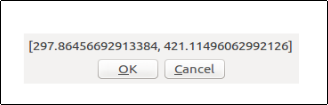
\includegraphics[width=10.0cm,trim=8 8 8 8,clip]{./images/disegnare/disegnare-28.png}
   \label{dis-28}
\end{figure}

\vskip 1cm

The two numbers between brackets represent the coordinates x and y of the position in the space of the page: 298 e 421\footnote{we approximated the two numbers to four significative digits, that are adequate to determine the position on the sheet, to aour goals.
In the following note we give a short explanation of the unit of measurement used for these numbers} respectively. Since we have just opened the document and that at the beginning the turtle is placed in the centre, we can assume that these coordinates represent the centre of the page. Nevertheless, in order to have the complete control of the situation, we need to know exactly the extension of the image's space. Now, the coordinates of the upper left angle are [0, 0], where the first number represents the coordinate x and the second the y, whilst those in the lower right angle are easily obtained by printing the value of the special variable \textbf{PAGESIZE}, that LibreLogo uses to mantain the page's dimensions. In this moment my version of Writer is set for pages A4 and, consequently, by executing the instruction

\vskip 1cm

\begin{scriptsize}
\begin{minipage}{1.0\textwidth}
\begin{itemize}[itemsep=-3pt,parsep=2pt]
\item[] \textbf{PRINT PAGESIZE}
\end{itemize}
\end{minipage}
\end{scriptsize}

\vskip 1cm

we obtain:

\vskip 1cm

\begin{figure}[H]
   \centering
   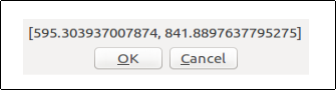
\includegraphics[width=10.0cm,trim=8 8 8 8,clip]{./images/disegnare/disegnare-29.png}
   \label{dis-29}
\end{figure}

\vskip 1cm

These numbers, rounded up, 596 and 842, represent the dimensions of a A4 sheet expressed in "points" at the density of 72 DPI/footnote{The acronym DPI stands for dots per inch. The value of DPI depends on the physical support over which an image is supposed to be represented.
Since an inch is 2.54 cm, 72 DPI density corresponds to 72/2.54 = 28.3 points for cm, or 2.83 points for mm; just to have a more familiar reference. When in Writer you choose the measurement unit "points" (instead of cm or inches), these refer to the density of 72 DPI just cited. In Writer, the measurement unit can be changed by clicking Tools->Options->LibreOffice Writer->General. you can choose between mm, cm, inches, pica, points.}. In mm it will be 210 and 297 mm. Let's recap the situation with the following picture.

\vskip 1cm

\begin{figure}[H]
   \centering
   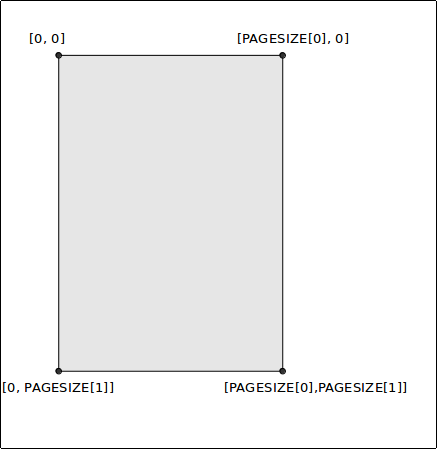
\includegraphics[width=10.0cm,trim=8 8 8 8,clip]{./images/disegnare/disegnare-30.png}
   \label{dis-30}
\end{figure}

\vskip 1cm

Every time we want to use absolute positions we can refer to this scheme that gives us the orientation of the referral system onthe sheet and its dimensions. In the next chart we can see the equivalent numeric values:

\begin{center}
%\begin{tabular}{| >{\centering\arraybackslash}m{1in} | >{\centering\arraybackslash}m{1in} |}
\begin{tabular}{| l | l |}
\hline
[0, 0] & [0, 0] \\ \hline
[PAGESIZE[0], 0]  & [596, 0] \\ \hline 
[0, PAGESIZE[1]]  &     [0, 842]   \\ \hline 
[PAGESIZE[0], PAGESIZE[1]]  & [596, 842]   \\ \hline 
\end{tabular}
\end{center}

Reconnecting to the previous paragraph, PAGESIZE is a variable, a variable that inside LibreLogo is treated as a constant because it contains the dimensions of a page. Besides it's that particular kind of variable that is called vector, because it's composed by more elements, precisely two, the two dimensions of the page: PAGESIZE[0] is the width and PAGESIZE[1] the lenght.
Come facciamo dunque per spedire la tartaruga in una posizione precisa?

\vskip 1cm

\begin{figure}[H]
   \centering
   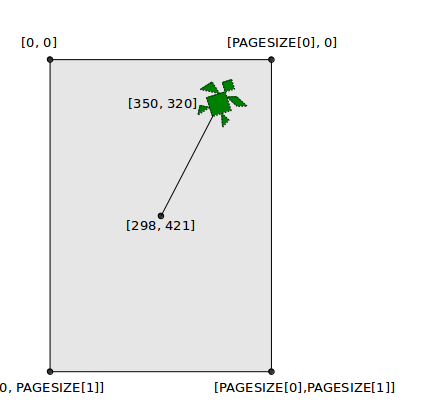
\includegraphics[width=10.0cm,trim=8 8 8 8,clip]{./images/disegnare/disegnare-31.png}
   \label{dis-31}
\end{figure}

\vskip 1cm

With the instruction \textbf{POSITION [350, 320]} the turtle moves directly to the coordinates point \textbf{POSITION [[350,320]}, 
starting from the point where it is, in this case from the centre of the page.
As can we use the instruction POSITION to control the position, in the same way we can use the instruction HEADING to control the direction where the turtle is heading. Evoking the instruction HEADING without any parameter we obtain the  current position.
By using another parameter, for instance HEADING [30], we make the turtle rotate by 30\degree. 
In the next picture we show the orientation of the reference system.

\vskip 1cm

\begin{figure}[H]
   \centering
   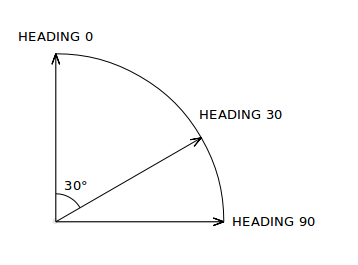
\includegraphics[width=10.0cm,trim=8 8 8 8,clip]{./images/disegnare/disegnare-32.png}
   \label{dis-32}
\end{figure}

\vskip 1cm

When we open a nwe document, or after the instruction HOME, the turtle points towards the upper side of the sheet, and this direction corresponds to 0\degree.

\subsection{More graphics commands}

It's possible to control other aspects of the drawing as well, in addition to the colour.

\subsubsection{PENWIDTH (pen thickness)}

With the command \textbf{PENWIDTH} we determine the thickness of the line:

\vskip 1cm

\begin{figure}[H]
   \centering
   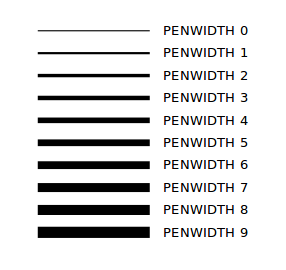
\includegraphics[width=10.0cm,trim=8 8 8 8,clip]{./images/disegnare/disegnare-33.png}
   \label{dis-33}
\end{figure}

\vskip 1cm

\subsubsection{PENJOINT (extremities shape)}

With the command \textbf{PENJOINT} we controll the vertexes form: 

Let's draw a triangle, for example, in the following way:

\vskip 1cm

\begin{scriptsize}
\begin{minipage}{0.40\textwidth}
\begin{itemize}[itemsep=-3pt,parsep=2pt]
\item[] PENWIDTH 5           
\item[] FORWARD 40 RIGHT 120
\item[] FORWARD 40 RIGHT 120
\item[] FORWARD 40 RIGHT 120
\item[] HIDETURTLE
\end{itemize}
\end{minipage}
\end{scriptsize}
\begin{minipage}{0.4\textwidth}
\begin{figure}[H]
   
\includegraphics[width=3.0cm,trim=4 4 8 4,clip]{./images/disegnare/disegnare-34.png}
   \label{dis-34}
\end{figure}
\end{minipage} \hfill

\vskip 1cm

We can alter the vertexes overlay by giving the instruction PENJOINT and an appropriate argument. Le possibilities are the following:

\vskip 1cm

\begin{figure}[H]
   \centering
   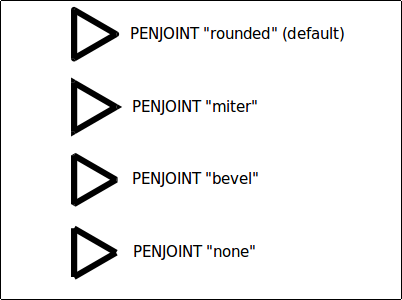
\includegraphics[width=10.0cm,trim=8 8 8 8,clip]{./images/disegnare/disegnare-35.png}
   \label{dis-35}
\end{figure}

\vskip 1cm

The argument "rounded" (default) mustn't be written in the command: we added it to point out that that is the standard behavoiur if anything else is specified. If however we just used one of the other options, then it has to be used explicitly the command \textbf{PENJOINT  "rounded "}, to obtain rounded vertexes. The argument "miter" stands for "........", that is what's realized when one cuts the frames cutting the straight edges so that the vertexes end up pointed.
per ottenere i vertici arrotondati. L'argomento  "miter " significa  "mitria " e sta peer  "giunto a mitria ", o  "giunto a quartabono ", che è quello che si realizza nelle cornici dei quadri tagliano i singoli regoli della cornice in maniera che i vertici risultino a punta.  "bevel " significa vertici smussati.

\subsubsection{PENCAP (it forms extremities of segments)}

With this command you can control the ends of a segment:

\vskip 1cm

\begin{figure}[H]
   \centering
   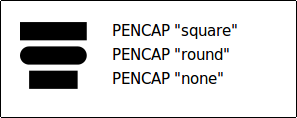
\includegraphics[width=10.0cm,trim=8 8 8 8,clip]{./images/disegnare/disegnare-36.png}
   \label{dis-36}
\end{figure}

\vskip 1cm

To comment this command behaviour, and also to recap code writing in Logo, let's analize the code used to produce this drawing, omitting, for the sake of simplicity, the part that produces the writing on the right. To understand more easily, let's orient ourselves with cardinal points, so orientated:

\vskip 1cm

\begin{figure}[H]
   \centering
   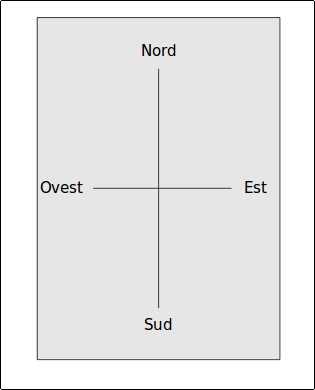
\includegraphics[width=10.0cm,trim=8 8 8 8,clip]{./images/disegnare/disegnare-37.png}
   \label{dis-37}
\end{figure}

\vskip 1cm

Let's see the following code:

\pagebreak

\vskip 1cm

%https://en.wikibooks.org/wiki/LaTeX/Source_Code_Listings
\lstset{literate=
  {á}{{\'a}}1 {é}{{\'e}}1 {í}{{\'i}}1 {ó}{{\'o}}1 {ú}{{\'u}}1
  {Á}{{\'A}}1 {É}{{\'E}}1 {Í}{{\'I}}1 {Ó}{{\'O}}1 {Ú}{{\'U}}1
  {à}{{\`a}}1 {è}{{\`e}}1 {ì}{{\`i}}1 {ò}{{\`o}}1 {ù}{{\`u}}1
  {À}{{\`A}}1 {È}{{\'E}}1 {Ì}{{\`I}}1 {Ò}{{\`O}}1 {Ù}{{\`U}}1
  {ä}{{\"a}}1 {ë}{{\"e}}1 {ï}{{\"i}}1 {ö}{{\"o}}1 {ü}{{\"u}}1
  {Ä}{{\"A}}1 {Ë}{{\"E}}1 {Ï}{{\"I}}1 {Ö}{{\"O}}1 {Ü}{{\"U}}1
  {â}{{\^a}}1 {ê}{{\^e}}1 {î}{{\^i}}1 {ô}{{\^o}}1 {û}{{\^u}}1
  {Â}{{\^A}}1 {Ê}{{\^E}}1 {Î}{{\^I}}1 {Ô}{{\^O}}1 {Û}{{\^U}}1
  {œ}{{\oe}}1 {Œ}{{\OE}}1 {æ}{{\ae}}1 {Æ}{{\AE}}1 {ß}{{\ss}}1
  {ű}{{\H{u}}}1 {Ű}{{\H{U}}}1 {ő}{{\H{o}}}1 {Ő}{{\H{O}}}1
  {ç}{{\c c}}1 {Ç}{{\c C}}1 {ø}{{\o}}1 {å}{{\r a}}1 {Å}{{\r A}}1
  {€}{{\euro}}1 {£}{{\pounds}}1 {«}{{\guillemotleft}}1
  {»}{{\guillemotright}}1 {ñ}{{\~n}}1 {Ñ}{{\~N}}1 {¿}{{?`}}1
}
\lstset{extendedchars=true, basicstyle=\scriptsize} 
\begin{lstlisting}[frame=single]  % Start your code-block

CLEARSCREEN		; I cancel the sheeet (just the graphic part)
HOME			; starting point: turtle in the center, pointing North 
HIDETURTLE		; I hide the turtle 
PENWIDTH 15		; I set the thickness of the line at 15 pt

RIGHT 90		; I rotate 90\degree to the right so the turtle can 
			; points towards East so that
			; to mark from left to right
				
PENCAP  "square "		; I set the mode "squares ends"
FORWARD 40		; I draw 40 pt of line
			; (Ovest -> Est)
PENUP  			; I lift the pen
RIGHT 90 FORWARD 20	; I turn right by 90\degree (pointing South) and 
			; I decrease by 20 pt
LEFT 90 BACK 40		; I turn left (pointing East) and I get back
			; back  (East -> West) by 40 pt
PENDOWN			; I put down the pen

PENCAP  "round "	; I set the mode "rounded ends"
FORWARD 40		; I draw 40 pt of line
			; (West -> East)
PENUP			; I lift the pen
RIGHT 90 FORWARD 20	; I turn right by 90\degree (pointing South) and
			; I decrease by 20 pt
LEFT 90 BACK 40		; I turn left (pointing East), I get back 
			; back ( East -> West) by 40 pt 
PENDOWN			; I put down the pen

PENCAP  "none "		; I set the mode "rounded ends"
FORWARD 40		; I draw 40 pt of line
			; (West -> East)
PENUP			; I lift the pen

\end{lstlisting}

\vskip 1cm

We highlighted the instructions that realize three traits, here reported:

\vskip 1cm

\begin{figure}[H]
   \centering
   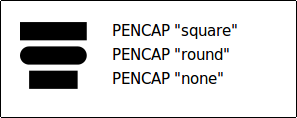
\includegraphics[width=10.0cm,trim=8 8 8 8,clip]{./images/disegnare/disegnare-36.png}
   \label{dis-38}
\end{figure}

\vskip 1cm

There, it's clear that in reality all three are drawn with the same lenght of 40 pt, and instead they don't seem to be the same lenght.
This is to understand how the command PENCAP works. The line drawn without specifications for the ends ("none effect) is 40 pt long.
So those with "round" and "square" effects" come out longer. It's clear that roundings are added to the normal lenght and that the "square" effect is obtained by straightening the roundings.

I's evident that this is just a marginal aspect. We took the opportunity to show the extreme sophistication of LibreLogo, to get used to move in the sheet and think graphically.

\subsubsection{PENSTYLE (dashed segments)}

With this instruction you can define the continuity of the trace, to produce dashed lines of many kinds:

\vskip 1cm

\begin{figure}[H]
   \centering
   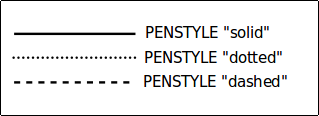
\includegraphics[width=10.0cm,trim=8 8 8 8,clip]{./images/disegnare/disegnare-38.png}
   \label{dis-39}
\end{figure}

\vskip 1cm

It's also possible to adjust the trace. For example with the instruction \textbf{PENSTYLE [3, 1mm, 2, 4mm, 1mm]} we obtain the trace:

\vskip 1cm

\begin{figure}[H]
   \centering
   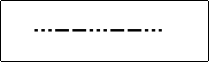
\includegraphics[width=10.0cm,trim=8 8 8 8,clip]{./images/disegnare/disegnare-39.png}
   \label{dis-40}
\end{figure}

\vskip 1cm

These are the rules: 

\begin{itemize}
\item Parametro 1: numeber of points
\item Parametro 2: lenght of points
\item Parametro 3: number of traits
\item Parametro 4: lenght of traits
\item Parametro 5: lenght of spaces
\item Parametro 6: optional, if it's worth 2 then the rectangles are forced to squares 
\end{itemize}

\subsubsection{FILLSTYLE (cross-hatchinga)}

The instruction FILLSTYLE 1, prior to the drawing of a figure, determines the trait of it. The numeric parameter determins the trait style, in the following way: 


\vskip 1cm

\begin{figure}[H]
   \centering
   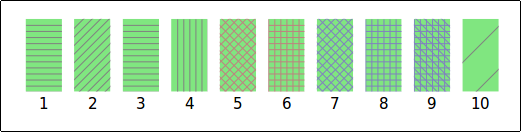
\includegraphics[width=10.0cm,trim=8 8 8 8,clip]{./images/disegnare/disegnare-40.png}
   \label{dis-41}
\end{figure}

\vskip 1cm

Here as well, it's possible to personalize the trait scheme, using additional parameters:

\vskip 1cm

\begin{scriptsize}
\begin{minipage}{0.50\textwidth}
\begin{itemize}[itemsep=-3pt,parsep=2pt]
\item[] \textbf{FILLSTYLE [2,  "red ", 3pt, 15\degree]}           
\end{itemize}
\end{minipage}
\end{scriptsize}
\begin{minipage}{0.3\textwidth}
\begin{figure}[H]
   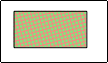
\includegraphics[width=3.0cm,trim=4 4 8 4,clip]{./images/disegnare/disegnare-41.png}
   \label{dis-42}
\end{figure}
\end{minipage} \hfill

\vskip 1cm

\subsection{Conclusioni}

With these instructions the part of our LibreLogo exploration dedicated to drawing ends. We learnt the main commands to move the turtle through the sheet, both to draw or and simply move. We learnt to move how a real turtle would, or the way we would do when we follow a path around our city, following a certain path, imagining a "forward" in front of our current position, a "backward", a right and a left. But we also saw how to move with a "teleportation", as if setting our car's nav sat would instantly propel us into that place, without having to go through the ends of the Earth; or how the knight moves in a chess game, jumping directly to its destination square distant 1+2 or 2+1 positions. We saw how to code colours to decorate both the lines and the surfaces. Knowing all this gave us the impression that we can manage everything on the sheet, but then we suddenly discovered some instructions to draw directly le main geometrical figures: squares, rectangles, circles and ellipses, with some variables, like sectors, segments and arches of ellipese (or circles), or rectangles with rounded edges. So we introduced the first of the fundamental elements that characterise a real programming language: the concept of variable, with which we can use generic literary symbols to design specific quantities - distances, angles and more - without having to worry about giving them precise numeric values; an essential characteristic that confers the language a potential similar to that being at the foundation of algebra, with symbolic calculus. We haven't exploredall the potential that underlies to the concept of variable, but just underlined what we needed to outline the movements on the sheet based on the use of spatial coordinates. To do so we had to consider a particular type of variable that is the vector, made itself by more numbers - two if it's the case of a "position vector" on a surface. Finally we saw that we can use many other commands to determine the specific graphics of the trait (colour, width, ends, junctions) and of the surfaces (colour, dotted lines). At this point, again, we may seem to have at our disposal a powerful instrument to produce graphics to insert in documents. And actually many things can be undoubtedly done with the commands we have seen so far. In fact, from the programming language point of view, we only saw a tiny part of its potential. These constructs, at the base of all programming languages, confer extraordinary capacities of flexibility and generalization to the countless kinds of software we all know, and unwittingly use in any device.

















